\documentclass[a4paper,10pt,twoside]{article}

\usepackage[top=1in, bottom=1in, left=1in, right=1in]{geometry}
\usepackage[utf8]{inputenc}

\usepackage{fancyhdr}
\usepackage{graphicx}

%\usepackage{lastpage}


%%%%%%%%%% Configuración de Fancyhdr - Inicio %%%%%%%%%%
\pagestyle{fancy}
\thispagestyle{fancy}
\lhead{TP2, Sistemas Operativos}
\renewcommand{\footrulewidth}{0.4pt}
\cfoot{\thepage /\pageref{LastPage}}

\fancypagestyle{caratula} {
   \fancyhf{}
   \cfoot{\thepage /\pageref{LastPage}}
   \renewcommand{\headrulewidth}{0pt}
   \renewcommand{\footrulewidth}{0pt}
}

%%%%%%%%%% Macros de tikz - Fin %%%%%%%%%%


\begin{document}


%%%%%%%%%%%%%%%%%%%%%%%%%%%%%%%%%%%%%%%%%%%%%%%%%%%%%%%%%%%%%%%%%%%%%%%%%%%%%%%
%% Carátula                                                                  %%
%%%%%%%%%%%%%%%%%%%%%%%%%%%%%%%%%%%%%%%%%%%%%%%%%%%%%%%%%%%%%%%%%%%%%%%%%%%%%%%


\thispagestyle{caratula}

\begin{center}


\includegraphics[height=2cm]{DC.png} 
\hfill

\includegraphics[height=2cm]{UBA.jpg} 

\vspace{2cm}

Departamento de Computación,\\
Facultad de Ciencias Exactas y Naturales,\\
Universidad de Buenos Aires

\vspace{4cm}

\begin{Huge}
TP2 - Pthreads
\end{Huge}

\vspace{0.5cm}

\begin{Large}
Sistemas Operativos
\end{Large}

\vspace{1cm}

Primer Cuatrimestre de 2016

\vspace{4cm}

\vspace{0.5cm}

\begin{tabular}{|c|c|c|}
\hline
Apellido y Nombre & LU & E-mail\\
\hline
Casanova, Manuel			& 355/05 & morbous$\_$panda@hotmail.com\\
Tripodi, Guido			& 843/10 & guido.tripodi@hotmail.com\\
\hline
\end{tabular}

\end{center}

\newpage


%%%%%%%%%%%%%%%%%%%%%%%%%%%%%%%%%%%%%%%%%%%%%%%%%%%%%%%%%%%%%%%%%%%%%%%%%%%%%%%
%% Índice                                                                    %%
%%%%%%%%%%%%%%%%%%%%%%%%%%%%%%%%%%%%%%%%%%%%%%%%%%%%%%%%%%%%%%%%%%%%%%%%%%%%%%%


\tableofcontents

\newpage


%%%%%%%%%%%%%%%%%%%%%%%%%%%%%%%%%%%%%%%%%%%%%%%%%%%%%%%%%%%%%%%%%%%%%%%%%%%%%%%
%% Desarrollo                                                                %%
%%%%%%%%%%%%%%%%%%%%%%%%%%%%%%%%%%%%%%%%%%%%%%%%%%%%%%%%%%%%%%%%%%%%%%%%%%%%%%%

\newpage
\section{Desarrollo y Resultados}

\section{Parte I – Desarrollo de Read-Write Lock}


\subsection{Ejercicios}
\begin{itemize}
 \item \textbf{Ejercicio 1 } Programar un tipo de tarea TaskConsola, que simular\'{a} una tarea interactiva.
La tarea debe realizar n llamadas bloqueantes, cada una de una duraci\'{o}n al azar 1 entre bmin
y bmax (inclusive). La tarea debe recibir tres par\'{a}metros: n, bmin y bmax (en ese orden)
que ser\'{a}n interpretados como los tres elementos del vector de enteros que recibe la funci\'{o}n.
Explique la implementaci\'{o}n realizada y grafique un lote que utilice el nuevo tipo de tarea.
\item \textbf{Ejercicio 2} El grupo de competencia de Data Mining, reciente ganador de importante concurso internacional, esta
preparando el algoritmo para su próxima victoria. Para esto necesita utilizar fuertemente la CPU por 500 ciclos.
A su vez, el grupo usa la máquina como servidor remoto, utilizando 3 usuarios que realizan llamadas bloqueantes de 10, 20 y 30 
respectivamente y de una duración al azar de hasta 4 ciclos.
Escribir el lote de tareas que simule la situación del grupo. Ejecutar y graficar la simulación usando el algoritmo FCFS para 1 y 2 y 4 
núcleos con un cambio de contexto de 5 ciclos. Calcular la latencia de cada tarea en los dos gráficos. Explicar 
que desventaja tendría si debe mantener este algoritmo de scheduling y solo tiene disponible una computadora con un núcleo (haga
referencia a los gráficos y a los cálculos anteriores para justificar su explicación).

\item \textbf{Ejercicio 3} Programar un tipo de tarea TaskBatch que reciba dos par\'{a}metros: total cpu y
cant bloqueos. Una tarea de este tipo debera realizar cant bloqueos llamadas bloqueantes, en
momentos elegidos pseudoaleatoriamente. En cada tal ocasi\'{o}n, la tarea deber\'{a} permanecer
bloqueada durante exactamente dos (4) ciclos de reloj. \\
El tiempo de CPU total que utilice una
tarea TaskBatch deber\'{a} ser de total cpu ciclos de reloj (incluyendo el tiempo utilizado para
lanzar las llamadas bloqueantes; no as\'{i} el tiempo en que la tarea permanezca bloqueada).
Explique la implementaci\'{o}n realizada y grafique un lote que utilice 4 tareas TaskBatch con
par\'{a}metros diferentes y que corra con el scheduler FCFS.
\end{itemize}

\subsection{Resultados y Conclusiones}

\subsubsection[Resolución Ejercicio 1]{Ejercicio 1}

\indent Dada la simpleza del código, optamos por mostrar nuestra implementación, en vez de comentarlo\\ detalladamente.\\
\indent Realizamos un ciclo de i \textless \ params[0], donde utilizamos la función dada por la catedra, uso\_IO a la cual le pasamos
el pid correspondiente y un entero ciclos que es el valor random obtenido entre $bmin$ y $bmax$. Esa función uso\_IO simula una llamada bloqueante.
\begin{center}
 \begin{verbatim}
                     ciclos = rand() % (params[2] - params[1] + 1) + params[1];
 \end{verbatim}

\end{center}

\indent A continuaci\'{o}n, el c\'{o}digo mencionado:

\begin{verbatim}

                  void TaskConsola(int pid, vector<int> params) {
                       int i, ciclos;              
                       for (i = 0; i < params[0]; i++) {
                              ciclos = rand() % (params[2] - params[1] + 1) + params[1];  
                              uso_IO(pid, ciclos);
                       }
                  } 

\end{verbatim}

\indent Como experimentaci\'{o}n trabajamos con el siguiente lote:\\

\begin{verbatim}
                              TaskConsola 5 3 7
                              TaskConsola 2 3 3
                              TaskConsola 15 2 7
\end{verbatim}

De aqu\'{i}, obtuvimos los siguientes resultados:\\

\vspace*{0.3cm} \vspace*{0.3cm}
  \begin{center}
 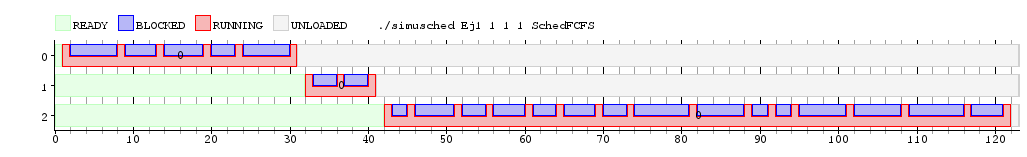
\includegraphics[scale=0.5]{./Test/ej1.png}
 { $Gr$\'a$fico \ 1.1$ Scheduler FCFS - 1 core }
 \end{center}
  \vspace*{0.3cm}



\subsubsection[Resolución Ejercicio 2]{Ejercicio 2}

\indent Para este punto, utilizamos el siguiente lote de tareas:
\begin{verbatim}
 
                                     TaskCPU 500
                                     TaskConsola 10 2 4
                                     TaskConsola 20 2 4
                                     TaskConsola 30 2 4


\end{verbatim}

\indent El mismo, presenta una tarea de uso intensivo $TaskCPU$ que dura 500 ticks, y otras tres interactivas, las cuales se
bloquean 10, 20 y 30 veces respectivamente con una duración de entre 2 y 4 tanto para la primera, la segunda como la tercera.\\
A continuación, los respectivos gráficos de mediciones.


\vspace*{0.3cm} \vspace*{0.3cm}
  \begin{center}
 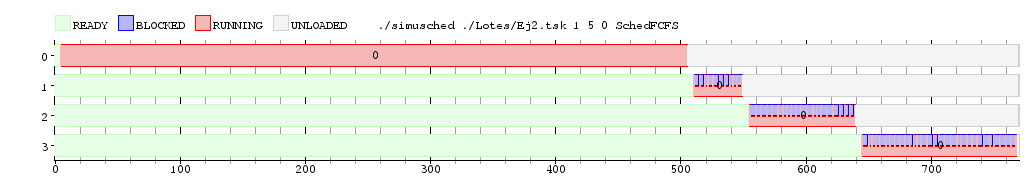
\includegraphics[scale=0.5]{ej21nucleo.png}
 { $Gr$\'a$fico \ 2.1$ Scheduler FCFS - 1 core }
 \end{center}
  \vspace*{0.3cm}
 
  
\vspace*{0.3cm} \vspace*{0.3cm}
  \begin{center}
 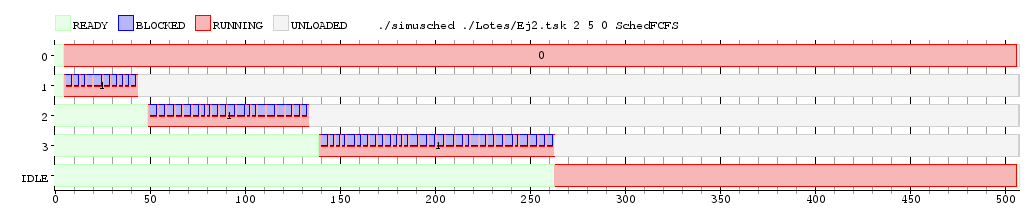
\includegraphics[scale=0.5]{ej22nucleo.png}
 { $Gr$\'a$fico \ 2.2$ Scheduler FCFS - 2 core }
 \end{center}
  \vspace*{0.3cm}
  
  \vspace*{0.3cm} \vspace*{0.3cm}
  \begin{center}
 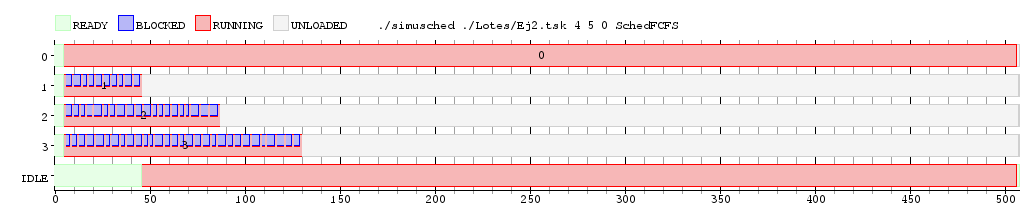
\includegraphics[scale=0.5]{ej24nucleo.png}
 { $Gr$\'a$fico \ 2.3$ Scheduler FCFS - 4 core }
 \end{center}
  \vspace*{0.3cm}

A su vez, se nos solicit\'{o} el c\'{a}lculo de la Latencia para cada una de las tareas bas\'{a}ndonos en la 
experimentaci\'{o}n con uno, dos y cuatro cores.\\

\textbf{Latencia:} Tiempo que demora una tarea en ejecutarse desde que la misma esta en estado $Ready$.\\

\indent Para el gr\'{a}fico uno, los valores obtenidos para cada tarea fueron los siguientes:\\

\begin{itemize}
 \item Tarea 0: 4
 \item Tarea 1: 510
 \item Tarea 2: 554
  \item Tarea 3: 644
\end{itemize}

\indent Para el gr\'{a}fico dos, los valores obtenidos para cada tarea fueron los siguientes:\\

\begin{itemize}
 \item Tarea 0: 4
 \item Tarea 1: 4
 \item Tarea 2: 49
  \item Tarea 3: 139
\end{itemize}

\indent Para el gr\'{a}fico tres, los valores obtenidos para cada tarea fueron los siguientes:\\

\begin{itemize}
 \item Tarea 0: 4
 \item Tarea 1: 4
 \item Tarea 2: 4
  \item Tarea 3: 4
\end{itemize}

\indent Se puede observar como aumenta el paralelismo a mayor cantidad de núcleos. 
En este scheduler en particular, esto ayuda de gran manera al rendimiento del sistema. Si el equipo
continuara usando el scheduler FCFS no podr\'{\i}a ejecutar otra tarea hasta que terminara de correr 
la anterior. Las consecuencias de este comportamiento son visibles en los 3 gr\'{a}ficos. Con un \'{u}nico core, 
solo se puede correr una tarea por vez, en este experimento comparado con usar 2 cores el tiempo se duplica.\\


\subsubsection[Resolución Ejercicio 3]{Ejercicio 3}


\indent Al igual que con la tarea TaskConsola, mencionaremos nuestro implementación y por consiguiente  
explicaremos ciertos puntos de la misma.\\
 \begin{verbatim}
                       void TaskBatch(int pid, vector<int> params) {
                            int total_cpu = params[0];
                            int cant_bloqueos = params[1];
                            vector<bool> uso = vector<bool>(total_cpu);
                            for(int i=0;i<(int)uso.size();i++) 
                               uso[i] = false;
                               for(int i=0;i<cant_bloqueos;i++) {
                                  int j = rand()%(uso.size());
                                  if(!uso[j])
                                     uso[j] = true;
                                  else
                                     i--; 
                               }
                               for(int i=0;i<(int)uso.size();i++) {
                                  if( uso[i] )
                                     uso_IO(pid,2); 
                                  else
                                     uso_CPU(pid, 1); 
                               }
                       }
 \end{verbatim}

 \indent Para este tipo de tarea, creamos un vector de tamaño igual a $total\_cpu$ el cual contiene valores booleanos, 
 si el valor en el \'{\i}ndice del vector es true este corresponder\'a a la funci\'{o}n uso\_IO, caso contrario uso\_CPU.\\
 Luego, utilizaremos un ciclo que irá desde 0 hasta el tamaño del vector y dependiendo el valor booleano, usará la funciones
 dadas por la catedra uso\_IO o uso\_CPU.\\
 
 \indent El experimento realizado para este nuevo tipo de tarea fue el siguiente:\\
 
 Con un lote de tareas:\\
 
 \begin{verbatim}
                           TaskBatch 3 3
                           TaskBatch 5 4
                           TaskBatch 4 4
                           TaskBatch 5 3
 \end{verbatim}

 Obtuvimos el siguiente diagrama:\\
 
 \vspace*{0.3cm} \vspace*{0.3cm}
  \begin{center}
 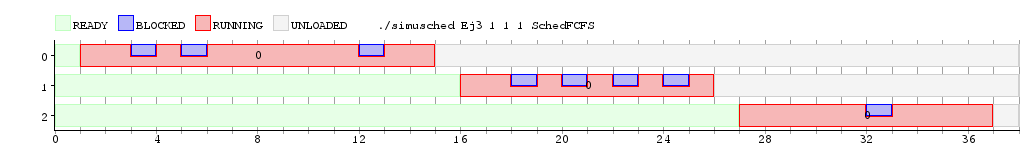
\includegraphics[scale=0.5]{ej3.png}
 { $Gr$\'a$fico \ 3.1$ Scheduler FCFS - 1 core }
 \end{center}
  \vspace*{0.3cm}
 

\newpage

\section{Parte II: RWLockTest}


\subsection{Ejercicios}
\begin{itemize}
 \item 
\textbf{Ejercicio 4}  Completar la implementación del scheduler Round-Robin implementando los
metodos de la clase SchedRR en los archivos sched rr.cpp y sched rr.h. La implementaci\'{o}n
recibe como primer par\'{a}metro la cantidad de n\'{u}cleos y a continuaci\'{o}n los valores de sus
respectivos quantums. Debe utilizar una \'{u}nica cola global, permitiendo ası la migraci\'{o}n de
procesos entre n\'{u}cleos.
\item \textbf{Ejercicio 5} Disene un lote con 3 tareas de tipo TaskCPU de 70 ciclos y 2 de tipo TaskConsola
con 3 llamadas bloqueantes de 3 ciclos de duraci\'{o}n cada una. Ejecutar y graficar la simulaci\'{o}n
utilizando el scheduler Round-Robin con quantum 2, 10 y 50.\\
Con un cambio de contexto de 2 ciclos y un solo n\'{u}cleo calcular la latencia, el waiting
time y el tiempo total de ejecuci\'{o}n de las cinco tareas para cada quantum. 
¿En cual es mejor cada uno? ¿Por qu\'{e} ocurre esto?
\item \textbf{Ejercicio 6} Grafique el mismo lote de tareas del ejercicio anterior para el scheduler FCFS.
Haciendo referencia a lo que se observa en los gr\'{a}ficos de este ejercicio y el anterior, explique
las diferencias entre un scheduler Round-Robin y un FCFS.
\item \textbf{Ejercicio 7} El scheduler SchedMistery fue creado por docentes investigadores de nuestra
materia y ha sido destacado en la ultima publicaci\'{o}n de ACM - SIGOPS, Operating Systems
Review. Desde entonces, numerosos investigadores de todo el mundo nos han contactado para
pedirnos su c\'{o}digo fuente. Sin embargo, su c\'{o}digo no aparece en ninguno de los repositorios
de la materia y nadie parece recordar quienes habıan estado detras de su implementaci\'{o}n.
Se les pide experimentar con dicho scheduler (aprovechando que hemos conseguido el c\'{o}di
go objeto) y replicar su funcionamiento en SchedNoMistery. Graficar como maximo tres lotes
de tareas utilizados en los experiementos y explicar en cada uno por separado que caracter\'{i}sticas
de SchedMistery identificaron con ese lote. Nota: El scheduler funciona para un solo
core y toma uno o mas argumentos num\'{e}ricos.
\item \textbf{Ejercicio 8} Implemente un scheduler Round-Robin que no permita la migraci\'{o}n de procesos
entre n\'{u}cleos (SchedRR2). La asignación de CPU se debe realizar en el momento en que se produce la carga 
de un proceso (load). El n\'{u}cleo correspondiente a un nuevo proceso ser\'{} aquel
con menor cantidad de procesos activos totales (RUNNING + BLOCKED + READY).Explique un escenario real 
donde la migraci\'{o}n de n\'{u}cleos sea beneficiosa y uno donde no (mencione
espec\'{i}ficamente que m\'{e}tricas de comparaci\'{o}n vistas en la materia mejorarıan en cada caso).
Disene un lote de tareas en nuestro simulador que represente a cada uno de esos escenarios
y grafique su resultado para cada implementaci\'{o}n. Calcule y compare en cada gr\'{a}fico las
m\'{e}tricas que menciono.

\end{itemize}


\subsection{Resultados y Conclusiones}

\subsubsection[Resolución Ejercicio 4]{Ejercicio 4}
Para desarrollar la implementación del scheduler $Round-Robin$ y que \'{e}ste funcione de una forma correcta
utilizamos una serie de estructuras puntuales. \\
Las mismas son las siguientes:\\
\begin{enumerate}
 \item Una cola global, la cual nombramos $q$, esta contiene los $PID$ de los procesos activos que no est\'{a}n
 bloqueados y en el tope de la misma se encuentra el próximo proceso a correr. Esta cola,
 fue desarrollada para que cuando se desaloje un proceso por finalizar su $quantum$ la misma pase al final de
 la cola y generando el ciclo acorde al comportamiento de este scheduler.
 \item Un vector denominado $cores$, este tiene en su elemento $i$ el pid correspondiente 
 al proceso que está corriendo en el core $i+1$. Inicializamos todos los elementos en -1, esto
corresponde a la Idle Task, de esta forma reconocemos que no se cargaron procesos en los núcleos.
\item Un vector $quantum$: el mismo guarda en la posici\'on $i$ el quantum que se dispuso a cada núcleo.
\item Un vector $quantumActual$ aqu\'{\i} guardaremos la cantidad de ticks que le quedan al proceso
desde que fue cargado en el core.
\item Una lista de $bloqueados$: esta tendr\'{a} los procesos que se bloquearon cuando estaban corriendo.
\end{enumerate}

Estas estructuras nos permiten determinar para cada tarea, cuándo, y cuánto 
de su quantum consumieron de forma que podamos desalojarla correctamente.\\

A su vez, tomamos ciertas decisiones en esta implementación:
\begin{itemize}
 \item Si una tarea se encuentra bloqueada cuando se produce el tick del reloj, misma es desalojada
de la cola global, y agregada en una lista de bloqueados. Además, ser\'{a} reseteado el quantum, se le
dará inicio a la próxima tarea que se encuentre ready y cuando el sistema operativo nos envie una
señal de unblock, la tarea desalojada regresará al final de la cola global.

\end{itemize}

\begin{center}

    
	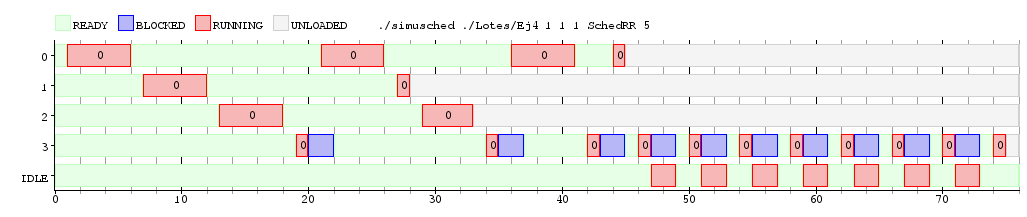
\includegraphics[width=450pt]{./Test/Ej4.png}
	{$Gr$\'a$fico 4.1 - Lote 1$ - Scheduler RR - 1 core - 5 quantum}	
 
\end{center}

Se puede ver en el gr\'{a}fico que cada 5 Ticks de reloj se cambia de tareas de manera c\'{\i}clica para mantener 
el fairness lo mas posible con todas las tareas. Salvo cuando una tarea se bloquea que esta es desalojada inmediatamente 
para no desperdiciar tiempo de computo esperando a que esta de desocupe.

\subsubsection[Resolución Ejercicio 5]{Ejercicio 5}

\indent El algoritmo de scheduler \textbf{Round-Robin} tiene como caracter\'istica asignar a todas las tareas 
un determinado tiempo m\'aximo de procesamiento, a esto se lo llama $quantum$. \\
\indent Este tiempo esta definido para cada n\'ucleo en particular, dependiendo de en cu\'al de ellos est\'en 
ejecutando los procesos, se les asignar\'a el respectivo tiempo m\'aximo.\\
\indent Otra caracter\'istica del \textbf{Round-Robin} es que las tareas se encolan y se ejecutan c\'iclicamente. 
Osea que cuando se deja de ejecutar, si no termin\'o su ejecuci\'on, la tarea se encolar\'a al final de la lista. 
Como elecci\'on de diseño, elegimos que se use una cola global para todos los procesadores, aunque tambi\'en
se podr\'ia tener una cola para cada n\'ucleo. \\
\indent A su vez, tambi\'en puede ocurrir una tarea no consuma todo su $quantum$. 
Ya sea porque la tarea se bloquea (haciendo uso de dispositivos de entrada/salida) o porque termine su ejecuci\'on.\\
\indent En caso de haber terminado, nuestro algoritmo pone a correr directamente la pr\'oxima tarea de acuerdo al orden 
circular que se estableci\'o y la tarea que finaliz\'o se desalojar\'a por completo y no sera considerada nuevamente. \\
\indent En caso de haberse bloqueado, esta misma dejar\'a de ser considerada hasta que se desbloquee, 
perdiendo el quantum que le quedaba si hubiere. 
Autom\'aticamente, seguir\'a corriendo la pr\'oxima tarea que se encuentre en la cola global. 
Cuando el proceso se desbloquee, ser\'a encolada nuevamente al final de dicha cola.   \\

\indent Para corroborar que el comportamiento era el deseado, nos solicitaron 1 lotes de tareas compuestos por tareas
del tipo $taskConsola$ y $taskCpu$, trabajando con 1 cores y utilizando distintos $quantum$ para cada uno de los mismos.\\


El lote de tareas fue el siguiente:
\begin{verbatim}
                                   *3 TaskCPU 70
                                   *2 TaskConsola 3 3 3
\end{verbatim}

Obteniendo los siguientes resultados:

\begin{center}

    
	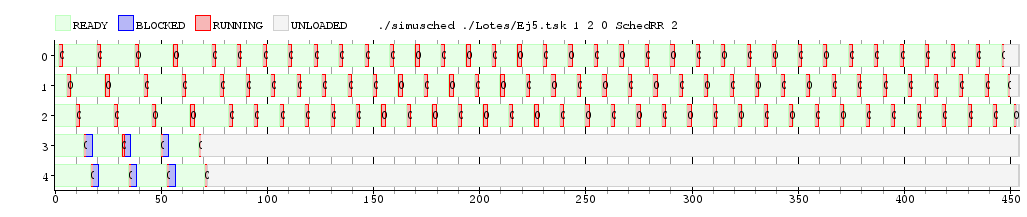
\includegraphics[width=450pt]{ej5quantum2.png}
	{$Gr$\'a$fico 5.1 Lote 1$ - Scheduler RR - 1 core - 2 quantum}	
 
\end{center}

\indent Latencia:\
\begin{itemize}
 \item Tarea 0: 1
 \item Tarea 1: 5
 \item Tarea 2: 9
 \item Tarea 3: 13
 \item Tarea 4: 16
 \item PROMEDIO: 8.8
\end{itemize}
\indent Waiting time:\
\begin{itemize}
 \item Tarea 0: 377
 \item Tarea 1: 380
 \item Tarea 2: 383
 \item Tarea 3: 59
 \item Tarea 4: 62
 \item PROMEDIO: 252.2
\end{itemize}
\indent Tiempo total de ejecuci\'{o}n:\
\begin{itemize}
 \item Tarea 0: 447
 \item Tarea 1: 450
 \item Tarea 2: 453
 \item Tarea 3: 69
 \item Tarea 4: 72
 \item PROMEDIO: 298.2
\end{itemize}

\begin{center}
  	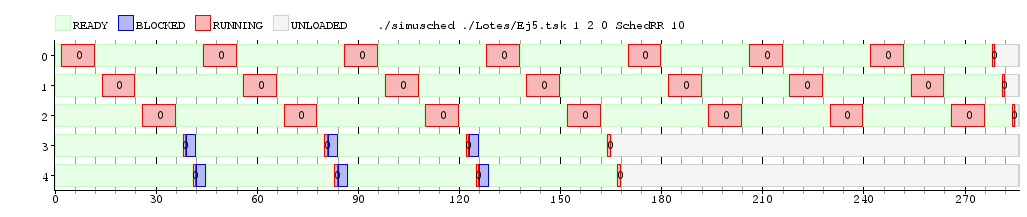
\includegraphics[width=450pt]{ej5quantum10.png}
	  {$Gr$\'a$fico 5.2 - Lote 1$ - Scheduler RR - 1 core - 10 quantum}	
\end{center}

\indent Latencia:\
\begin{itemize}
 \item Tarea 0: 2
 \item Tarea 1: 14
 \item Tarea 2: 26
 \item Tarea 3: 38
 \item Tarea 4: 41
 \item PROMEDIO: 24,2
\end{itemize}
\indent Waiting time:\
\begin{itemize}
 \item Tarea 0: 209
 \item Tarea 1: 212
 \item Tarea 2: 215
 \item Tarea 3: 155
 \item Tarea 4: 158
 \item PROMEDIO: 189.8
\end{itemize}
\indent Tiempo total de ejecuci\'{o}n:\
\begin{itemize}
 \item Tarea 0: 279
 \item Tarea 1: 282
 \item Tarea 2: 285
 \item Tarea 3: 165
 \item Tarea 4: 168
 \item PROMEDIO: 235.8
\end{itemize}

\begin{center}
  	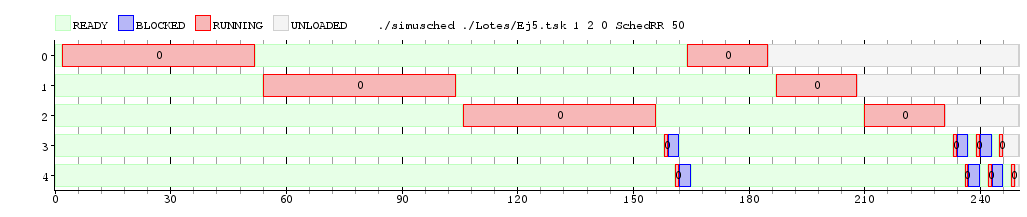
\includegraphics[width=450pt]{ej5quantum50.png}
	  {$Gr$\'a$fico 5.3 - Lote 1$ - Scheduler RR - 1 core - 50 quantum}	
\end{center}

\indent Latencia:\
\begin{itemize}
 \item Tarea 0: 2
 \item Tarea 1: 54
 \item Tarea 2: 106
 \item Tarea 3: 158
 \item Tarea 4: 161
 \item PROMEDIO: 96,2
\end{itemize}
\indent Waiting time:\
\begin{itemize}
 \item Tarea 0: 115
 \item Tarea 1: 138
 \item Tarea 2: 161
 \item Tarea 3: 236
 \item Tarea 4: 239
 \item PROMEDIO: 177.8
\end{itemize}
\indent Tiempo total de ejecuci\'{o}n:\
\begin{itemize}
 \item Tarea 0: 185
 \item Tarea 1: 208
 \item Tarea 2: 231
 \item Tarea 3: 246
 \item Tarea 4: 249
 \item PROMEDIO: 223.8
\end{itemize}

\indent
\begin{itemize}
 \item El caso con mejor latencia es el primer experimento, esto se debe al escaso quantum que se le otorga a cada tarea
 permitiendoles ejecutar por primera vez r\'{a}pidamente.
 \item El 3er experimento tiene el mejor waiting time, esto se debe a su alto quantum. Debido a que el quantum es muy elevado 
 se desperdicia la menor cantidad de ticks de reloj en cambio de contexto.
 \item Igual que en el caso anterior como el 3er experimento es el que menos ticks pierde por cambio de contexto debido al 
 alto quantum, esta es la que menos tiempo de ejecuci\'{o}n tiene.
\end{itemize}


\indent Se puede observar el cambio de tareas cíclico tanto porque terminaron su quantum o porque se bloquearon.\\


\indent Luego de estos experimentos pudimos observar ciertos puntos del comportamiento del Round-Robin:\\
\begin{itemize}
\item  Carácter circular del algoritmo.
\item  Desalojo de las tareas cuando se bloquean o terminan y la inmediata asignación del núcleo a la siguiente tarea en caso de existir alguna.
\item  Libre de inanición.
\item  Una tarea bloqueada es ignorada por el scheduler hasta que se desbloquee.
\end{itemize}

\indent Finalmente, dado su carácter circular y equitativo, podemos afirmar que todas las tareas que 
estén en condiciones de correr serán ejecutadas y ninguna será negada de tiempo de procesamiento.\\


\subsubsection[Resolución Ejercicio 6]{Ejercicio 6}

El lote de tareas solicitado fue el siguiente:
\begin{verbatim}
                                   *3 TaskCPU 70
                                   *2 TaskConsola 3 3 3
\end{verbatim}

Obteniendo los siguientes resultados:

\begin{center}
  	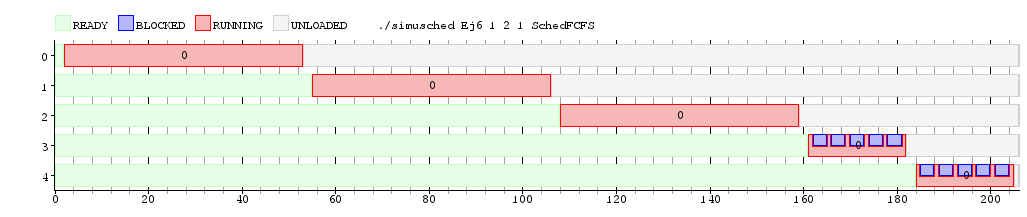
\includegraphics[width=450pt]{ej6.png}
	  {$Gr$\'a$fico 6.1 - Lote 1$ - Scheduler FCFS - 1 core}	
\end{center}

\indent A modo de an\'alisis, hemos obtenido las siguientes conclusiones:\\


\begin{itemize}
 \item Un scheduler FCFS corre una tarea hasta que esta termina a diferencia de uno Round-Robin 
que las va intercambiando otorg\'{a}ndole un tiempo equitativo a cada tarea.
\item Para que Round-Robin sea considerablemente mas eficiente que FCFS el quantum debe ser 
lo suficientemente alto para no tenes altos valores de waiting-time durante los cambios de 
contexto pero no demasiado alto sino se comporta igual que un scheduler FCFS.
\item Si se da el caso anterior el scheduler Round-Robin es eficiente en t\'{e}rminos 
de latencia en comparaci\'{o}n con FCFS.
\end{itemize}


\subsubsection[Resolución Ejercicio 7]{Ejercicio 7}

\indent En este punto se nos solicit\'{o} experimentar con el c\'{o}digo objeto de un 
SchedMistery y a partir de los mismos, realizar una r\'{e}plica del mismo.\\

A continuaci\'{o}n, expondremos tres experimentos de los cuales sacamos ciertas particularidades que presenta este Scheduler.\\

Con un lote de tareas compuesto por:\\

\begin{verbatim}
 @5:
TaskCPU 20
@0:
TaskCPU 7
TaskConsola 5 2 2
@:8
TaskConsola 4 2 3
\end{verbatim}

Obteniendo lo siguiente:
\begin{center}
    	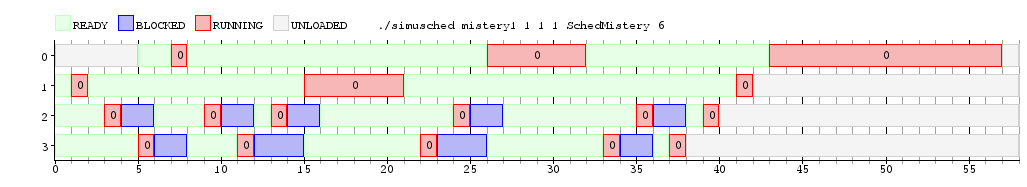
\includegraphics[width=450pt]{./Test/ej7_1.png}
	{$Gr$\'a$fico 7.1 - Lote 1$ - Sched Mistery - 1 core - Quantum = 6}	
 \end{center}
 
De aqu\'{\i}, pudimos deducir que una tarea al bloquearse es desalojada y cuando la misma se desbloquea, el scheduler, le da 
prioridad para que vuelva a correr.\\

Con el segundo lote:\\

\begin{verbatim}
TaskCPU 20
TaskConsola 20 4
TaskAlterno 1 1 1 1 1 1 15 1 1 1 1
\end{verbatim}

Obteniendo lo siguiente:
\begin{center}
    	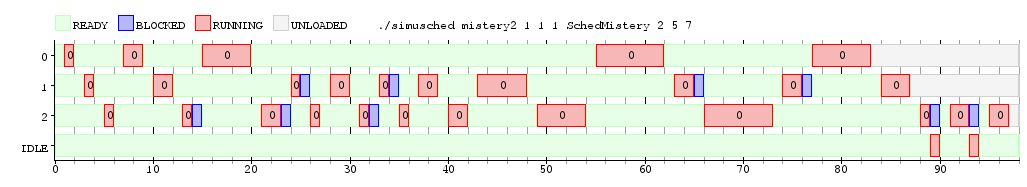
\includegraphics[width=450pt]{./Test/ej7_2.png}
	{$Gr$\'a$fico 7.2 - Lote 1$ - Sched Mistery - 1 core - Quantum = 2 - 5 - 7}	
 \end{center}

Con este lote lo primero que se observa es que los par\'{a}metros pasados al scheduler van a ser una lista de quantums 
donde cada tarea va a correr una \'{u}nica vez hasta el \'{u}timo quantum de la lista, y a partir de aquí siempre van a correr este. Adem\'{a}s esta lista siempre 
tiene un primer quantum de valor 1.\\
Tambi\'{e}n observamos que una tarea al desbloquearse vuelve a correr con el quantum anterior de la lista de los mismos. 
Las tareas cuando se desbloquean se les d\'{a} ''prioridad'' porque la prioridad es dada por el quantum que esta antes en 
la lista de quantums.\\

Con el siguiente lote:\\

\begin{verbatim}
              TaskCPU 20
              TaskCPU 10
              @20:
              TaskCPU 15
\end{verbatim}

Obteniendo lo siguiente:\\
\begin{center}
    	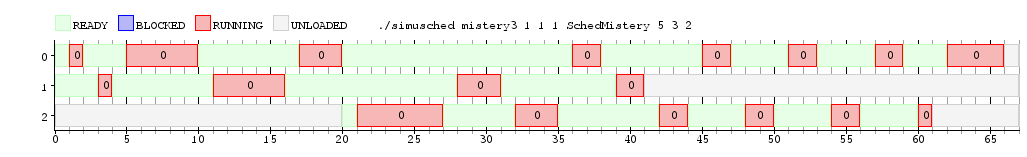
\includegraphics[width=450pt]{./Test/ej7_3.png}
	{$Gr$\'a$afico 7.2 - Lote 2$ - Sched Mistery - 1 core - Quantum = 5 3 2}	
 \end{center}
 
De aqu\'{\i}, pudimos observar, que si una tarea entra m\'{a}s tarde corre los quantums que ya pasaron de la lista. Esto da 
una noci\'{o}n de prioridad haciendo que estas tareas corran varias veces seguidas antes de que vuelva a correr otra.\\

\indent En conclusi\'on:\\


\begin{itemize}
 \item Se puede observar un caracter c\'{\i}clico con posibilidad de varios quantums distintos, los cuales van cambiando
 acorde a las vueltas c\'{\i}clicas que da el scheduler.
 \item Prioridad para tareas bloqueantes (al ser desbloqueada corren un quantum previo que tiene mayor prioridad)
 \item Prioridad para tareas m\'as recientes (Corren los quantums que ya pasaron de la lista hasta el quantum actual, esto 
 provoca que corra varias veces antes que sigan corriendo las tareas que entraron antes)
\end{itemize}

Para desarrollar la implementación del scheduler $No$ $Mistery$ y que este funcione de una forma correcta
utilizamos una serie de estructuras puntuales. \\
Las mismas son las siguientes:\\
\begin{enumerate}
\item Un entero $quantumActual$ en el cual almacenaremos el valor de quantum que tiene en el momento la tarea que esta corriendo.
\item Un vector de enteros llamado $quantum$, esta secuencia contiene en orden el valor de cada quantum pasado por par\'{a}metro.
\item Vector de colas de enteros de nombre $colasXQuantum$. Cada \'{i}ndice de la secuencia es una cola perteneciente a los quantum 
que se pasaron por par\'{a}metro. Estas colas tienen las tareas a ejecutar de cada quantum.
\item Un diccionario $pid$\_$quantum$ que dado el pid de una tarea me dice que quantum de la lista es el que tiene que correr.
\item Una funci\'{o}n auxiliar llamada $colasVacias$ que devuelve un valor booleano si no hay mas tareas en ninguna cola de los 
quantum.
\end{enumerate}

A continuación explicaremos por partes el c\'{o}digo de nuestro scheduler.\\

Cuando inicializa lo primero que hacemos mediante un ciclo for es guardar los quantums pasados por par\'{a}metro dentro de la 
secuencia $quantum$ y al mismo tiempo se van creando colas vacias en la secuencia $colasXQuantum$.\\

Cuando una nueva tarea es cargada esta se encola en el primer quantum de la lista y se crea una asociaci\'{o}n de dicha tarea 
con el número del quantum de la lista en el diccionario $pid$\_$quantum$.\\

En el momento en que una tarea se desbloquea nos fijamos cual fue el \'{u}ltimo quantum que corrió de la lista y si este no es 
el primero se la encola en la cola del quantum anterior, caso contrario se la encola en el mismo quantum que corrio la \'{u}ltima vez.
Por \'{u}ltimo se actualiza en caso de ser necesario la cola actual en el diccionario $pid$\_$quantum$.\\

En cada tick de reloj nos fijamos si la tarea termina, se bloquea o corre normalmente. En caso de que termine o se bloquee usamos 
la funci\'{o}n $next(cpu)$ ( mas adelante explicaremos que hace esta funci\'{o}n) para saber cual es la pr\'{o}xima 
tarea a correr. \\Si es un tick normal de reloj nos fijamos, si la tarea que esta corriendo es la IDLE, primero verificamos si hay 
alguna tarea encolada con la funci\'{o}n $colasVacias()$, en caso de haber al menos una devolvemos la pr\'{o}xima a ejecutar. Si 
no hay tareas seguimos corriendo la IDLE. Si la tarea que se esta ejecutando no es la IDLE restamos en uno el quantum y preguntamos 
si este llego a 0, en caso de no ser as\'{\i} se devuelve la misma tarea. Si este llego a 0 nos fijamos que quantum de la lista 
termino de correr, en caso de que no sea el \'{u}ltimo, se actualiza el dato en el diccionario $pid$\_$quantum$ con el siguiente y 
se encola en la cola correspondiente a este quantum y devolvemos la pr\'{o}xima tarea a ejecutar.\\

La funci\'{o}n $next(cpu)$ busca de todas las colas de los quantums cual es la primera que no este vac\'{\i}a, se saca el 
primer elemento de la cola y la funci\'{o}n lo devuelve. Adem\'{a}s guarda en la variable $quantumActual$ el quantum de la cola 
donde extrajimos la tarea.\\

Por \'{u}ltimo la funci\'{o}n $colasVacias()$ revisa todas las colas de los quantums y devuelve un valor booleano dependiendo si 
estan todas vacias (devuelve 1) o si hay alguna que contenga al menos una tarea en cuyo caso devuelve 0.\\


\subsubsection[Resolución Ejercicio 8]{Ejercicio 8}

La idea principal de esta nueva versi\'{o}n de $Round-Robin$ se centraliza en que no permita migraci\'{o}n entre
cores, esto se basa principalmente en utilizar una cola para cada núcleo por separado, y en cada
cola respectiva se encolar\'{a}n las tareas que fueron asignadas inicialmente a cada n\'ucleo.\\
Para desarrollar este tipo de algoritmo, el cual denominaremos $RR2$, utilizamos estructuras
puntuales, enunciadas a continuación:\\
\begin{itemize}
 \item Un vector $quantum$ y otro $quantumActual$, los cuales siguen cumpliendo la misma funci\'{o}n que
 en Round-Robin 1.
 \item Un vector de colas denominado $colas$, en el cual, en la posición $i$ encontraremos la cola correspondiente
 a ese núcleo de procesamiento.
 \item Un diccionario de $Bloqueados$, donde la clave contendr\'{a} el número de core, y en definición
 la tareas bloqueadas de ese core. Esto nos beneficiar\'{a} cuando haya que reubicarla en la cola de procesos ready.
 \item Un vector de enteros $cantidad$, que como la palabra lo define, tendrá en cada posición $i$ 
 la totalidad de las tareas, ya sea bloqueadas, activas o en estado ready que tiene asignado ese core, benefici\'{a}ndonos
 la determinación del núcleo al que se le asignará la tarea al momento de cargarla.
\end{itemize}
Cuando se carga una tarea, previamente, se chequeará que core tiene menor cantidad de procesos totales asignados (
aqu\'{\i} es donde el vector $cantidad$ entra en juego). Una vez que se obtiene este n\'{u}cleo, se agrega 
la tarea a la cola correspondiente y se actualiza la cantidad sumando una unidad.\\
\indent Al bloquearse un proceso, se define una nueva entrada en el diccionario $bloqueados$ con el
pid y el n\'{u}cleo correspondiente. De esta forma, al desbloquearse, colocamos la tarea en la cola del core
correspondiente y eliminamos la entrada del diccionario. Así logramos resolver el inconveniente de la nula
migración entre n\'{u}cleos.\\
\indent Finalmente, cuando una tarea finaliza, la quitamos y descontamos una unidad a la posición $i$ del vector
$cantidad$. Esta es la única vez, en la cual se descuenta. Aunque una tarea se bloquee, la misma
seguirá contando en el vector. De esta forma se cumplirá, que las tareas son asignadas a los cores
con menor cantidad de tareas.\\
Luego de realizar dicha implementación, en comparación al Round-Robin original, hemos conjeturado 
las siguientes hipótesis:

\begin{enumerate}
\item Comportamiento menos eficiente en el RR2 con respecto al paralelismo, ya que al no permitir
migración de n\'ucleos este se pierde.
\item Comportamiento más eficiente en el RR2 con lotes de tareas que se bloquean un gran n\'{u}mero
de veces. Esto surge ya que el Round-Robin original, es m\'as proclive a realizar cambios de contexto con la posibilidad
de darse un cambio de core.
\end{enumerate}
 
 Procedemos a demostrar la primer conjetura:\\
 
 \textbf{Comportamiento menos eficiente en el RR2 con respecto al paralelismo, ya que al no permitir
migración de núcleos este lo pierde}\\

Un ejemplo de esto, en la vida real ser\'ia, estar corriendo testeos de software y al mismo tiempo analizando
algoritmos de alta complejidad para demostraciones matem\'{a}ticas.\\

Un ejemplo de los lotes utilizados que demuestra esto fue el siguiente:\\

\begin{verbatim}
                                     TaskCPU 40
                                     TaskCPU 15
                                     TaskCPU 50
                                     TaskCPU 30
                                     TaskCPU 50
\end{verbatim}

Obteniendo los siguientes datos relevantes:\\

\begin{center}
    	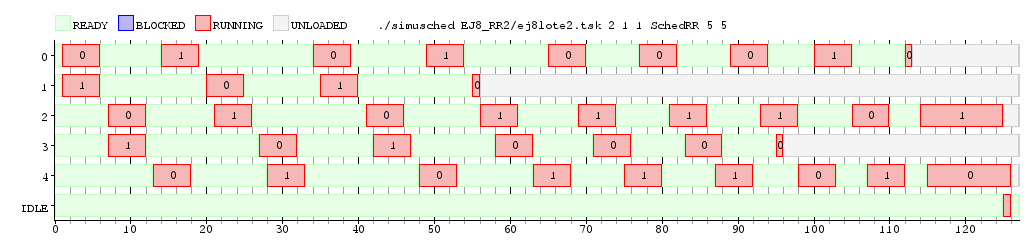
\includegraphics[width=450pt]{./EJ8_RR2/dif10corerr.png}
	{$Gr$\'a$fico 8.1 -Lote 3$ - Round Robin - 2 core - Quantum = 5 - cambio de contexto = 1}	
 \end{center}
 
 \begin{center}
    	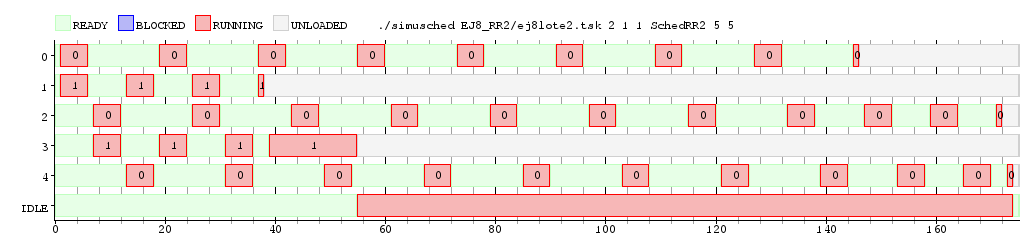
\includegraphics[width=450pt]{./EJ8_RR2/dif10corerr2.png}
	{$Gr$\'a$fico 8.2 - Lote 3$ - Round Robin 2 - 2 core - Quantum = 5 - cambio de contexto = 1}	
 \end{center}
 
 Se puede ver en estos diagramas como la implementación del Round Robin original trabaja
 mejor finalizando la ejecución de las tareas hasta 50 milisegundos antes.\\
 Esto se da por la falta de paralelismo de el RR2 ya que al ser asignados los procesos
 a cada core, cuando uno de los dos finaliza, este queda ocioso ya que no existe la
 posibilidad de migrar  procesos.\\
 
 Luego, el RR2 resulta beneficioso:
 
 \textbf{Comportamiento mas eficiente en el RR2 con lotes de tareas que se bloquean un gran numero
de veces}

\indent Un ejemplo de esto, puede ser al estar corriendo un juego (en el cual siempre se esta interactuando con el teclado) y
adem\'{a}s estar corriendo algun software.\\

Para esto,un lotes de tareas que ejemplifica lo dicho puede ser el siguiente:\\

\begin{verbatim}
                                     TaskCPU 40
                                     TaskBatch 10  5
                                     TaskCPU 50
                                     TaskBatch 15 8
                                     TaskCPU 10

\end{verbatim}


   \begin{center}
    	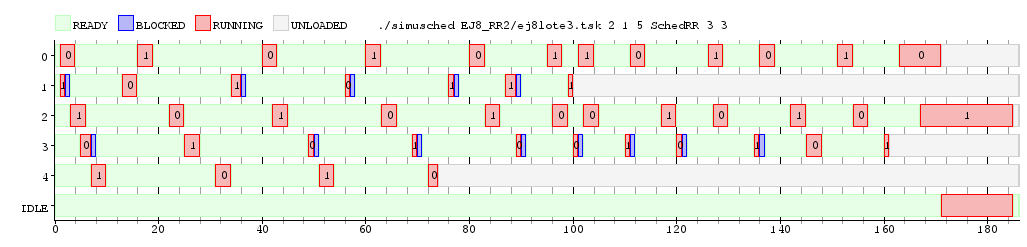
\includegraphics[width=450pt]{./EJ8_RR2/dif5corerr.png}
	{$Gr$\'a$fico 8.3 - Lote 3$ - Round Robin - 2 core - Quantum = 3 - cambio de contexto = 1}	
 \end{center}
 
 \begin{center}
    	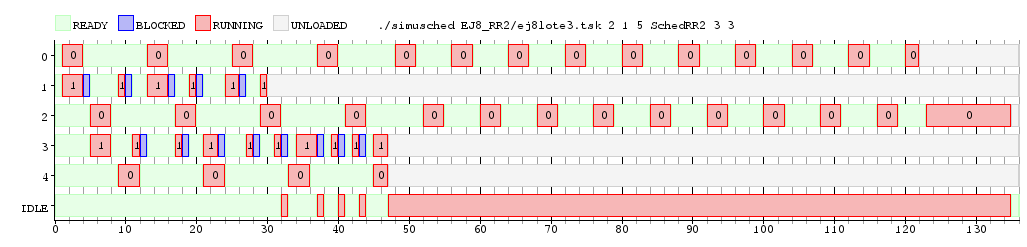
\includegraphics[width=450pt]{./EJ8_RR2/dif5corerr2.png}
	{$Gr$\'a$fico 8.4 - Lote 3$ - Round Robin 2 - 2 core - Quantum = 3 - cambio de contexto = 1}	
 \end{center}

 Se puede observar por los diagramas como el RR2 tiene una mejor performance en este estilo
 de lotes llegando a finalizar las ejecuciones hasta 50 milisegundos antes que el Round-Robin
 original.\\
 Como el Round-Robin original tiene pérdida de tiempo con el cambio de contexto y
 migración de tareas este empeora su performance en comparación al RR2 que no admite
 este tipo de migración es notorio la superioridad en relación a nuestra conjetura.\\
 
 Las m\'{e}tricas que m\'{a}s tuvimos en cuenta a la hora de analizar en que casos tiene mejor performance 
 cada scheduler fueron waiting time y turnaround. El turnaround ( tiempo de ejecuci\'{o}n es lo 
 que mas tomamos en cuenta a la hora de analizar la performance de ambos schedulers, cuanto mas r\'{a}pido 
 termine de ejecutar una tarea antes va a liberar al sistema para la siguiente tarea. Para analizar que t\'{a}n 
 r\'{a}pido se ejecuta una tarea se analiza el waiting time de las tareas en cada caso, una tarea con menos waiting 
 time tiene que esperar menos para volver a correr lo que va a reducir su tiempo de ejecuci\'{o}n.
 Podemos concluir luego de estas demostraciones que, el Round-Robin original es \'{a}mpliamente
 superior desde el punto de vista de la performance que se obtiene al trabajar con tareas
 que demanden mucho uso del CPU, mientras que el RR2 es \'{a}mpliamente mejor cuando se utilicen
 tareas que se bloqueen por un tiempo considerable.\\
 
 


\newpage

\section{Parte III: Desarrollo de Backend Multithreaded}


\subsection{Ejercicios}
\begin{itemize}
 \item 
\textbf{Ejercicio 3}
En segundo lugar, deberán implementar el servidor de backend multithreaded inspirándose en el código provisto y lo desarrollado en el punto anterior.
\end{itemize}

\subsection{Resultados y Conclusiones}


\subsubsection[Resolución Ejercicio 3]{Ejercicio 3}

\indent En este Ejercicio, se solicit\'{o} la implementación de un backend mutithreaded, para el desarrollo del mismo,
utilizamos la base del backend mono para la conexi\'{o}n con el servidor, el parseo de las fichas, tanto para la validez de las mismas
y tambi\'{e}n el env\'{\i}o de dimensiones del tablero de juego.\\

Utilizamos la función $atendedor\_de\_jugador$ la cual la convertimos en un thread para cada jugador. Esta función es llamada desde
la función main cuando las conexiones del socket entre el cliente-servidor son correctas. \\
Convertimos la función enunciada de la siguiente manera:\\
\begin{verbatim}
 pthread_create(&threads[i], NULL, &atendedor_de_jugador, &socketfd_cliente);
\end{verbatim}

En donde, threads es un arreglo de thread$\_$t y se le asigna uno a cada jugador y socketfd$\_$cliente es el atributo 
de cada thread. En este ejercicio como no vamos a necesitar el atributo todos los threads usan el mismo.

A continuación, mostraremos esta sección de código:\\
\begin{verbatim}
\*creacion de arreglo de threads *\

                      pthread_t threads[NUM_THREADS];
                      
\end{verbatim}

Luego, en la función $atendedor\_de\_jugador$ la cual recibe un thread$\_$data lo guardamos en un puntero a thread$\_$data llamado
my$\_$data y creamos un entero llamado socket$\_$fd el socket que nos viene como parametro.\\

Luego, basandonos en el backend mono, realizamos una implementación similar con la particularidad que, en el if donde se
consulta si el mensaje del jugador es una parte del barco, el barco terminado, una bomba o update.\\
En caso de ser una parte de barco, luego de parsear el casillero, y al chequear la validez de la ficha utilizamos nuestro read\_write\_lock y realizamos
la funcion $wlock()$. En caso de ser una ficha valida, realizamos un write lock y procedemos a escribir de la siguiente manera:\\
\begin{verbatim}
				(*rwlocks_tablero)[ficha.fila][ficha.columna].wlock();
				(*tablero_jugador)[ficha.fila][ficha.columna] = ficha.contenido;
				(*rwlocks_tablero)[ficha.fila][ficha.columna].wunlock();
                     
                     
\end{verbatim}
Para luego enviar la misma y terminar la jugada. En caso de que la validez de la ficha no sea correcta, dejamos de leer
y procedemos a escribir para quitar fichas y asi dejar de escribir.

Por consiguiente, en caso de que el mensaje sea una barco terminado se realiza un wlock para escribir la palabra y luego un wunlock.\\

El mismo se detalla a continuación:\\
\begin{verbatim}
			for (list<Casillero>::const_iterator casillero = barco_actual.begin(); casillero != barco_actual.end(); casillero++) {
				(*rwlocks_tablero)[casillero->fila][casillero->columna].wlock();
				(*tablero_jugador)[casillero->fila][casillero->columna] = casillero->contenido;
				(*rwlocks_tablero)[casillero->fila][casillero->columna].wunlock();
			}
			barco_actual.clear();       
\end{verbatim}

Luego, en caso de ser una bomba chequeamos si el casillero donde se coloco la bomba tiene un barco o una bomba, en caso de tener una bomba se envia el mensaje de que ya estaba golpeado como en el backend mono. Si había un barco, hacemos un wlock para escribir en el casillero bomba y liberamos el lock.\\

De esta manera, queda implementado nuestro backend multithreaded como fue solicitado.







\newpage

%%%%%%%%%%%%%%%%%%%%%%%%%%%%%%%%%%%%%%%%%%%%%%%%%%%%%%%%%%%%%%%%%%%%%%%%%%%%%%%
%% Conclusión                                                                %%
%%%%%%%%%%%%%%%%%%%%%%%%%%%%%%%%%%%%%%%%%%%%%%%%%%%%%%%%%%%%%%%%%%%%%%%%%%%%%%%

\newpage
\section{Bibliografía}

\begin{itemize}
 \item Cátedra de Sistemas Operativos - Clases teóricas y prácticas (1º Cuatrimestre 2016)
 \item The Little Book of Semaphores
\end{itemize}

\end{document}
